During the EDA we study properties of the entries of the tidy dataset.
In particular we focus on outlier detection, distribution of the features,
correlations between variables, principal components and clustering.
We also anticipate that we will not use the \texttt{solutions} and
\texttt{init} variables in the regression analysis and as such we do not
include them in the EDA as well: they only serve as labels for the
identification of the entries.

\subsection{Outliers Detection}\label{sec:eda:outliers}

We perform outliers detection using the definition of the
\textit{interquartile} range, typical in statistical analysis.
This is defined as the interval between the 25th and 75th percentile of the
sample distribution, and outlying samples are entries greater or lower than 1.5
times such interval with respect to the sample mean.

We apply this procedure for each column in the dataset and compute the average
quantity of outlying samples for each variable: the truncation levels hold
between 17\% and 27\% of outliers in their distributions, while \texttt{weight}
holds only 6\% of outliers with respect to its distribution (the \texttt{type}
feature is categorical and as such there is no point in studying the outlying
samples for it). 
\begin{figure}[htbp]
  \centering
  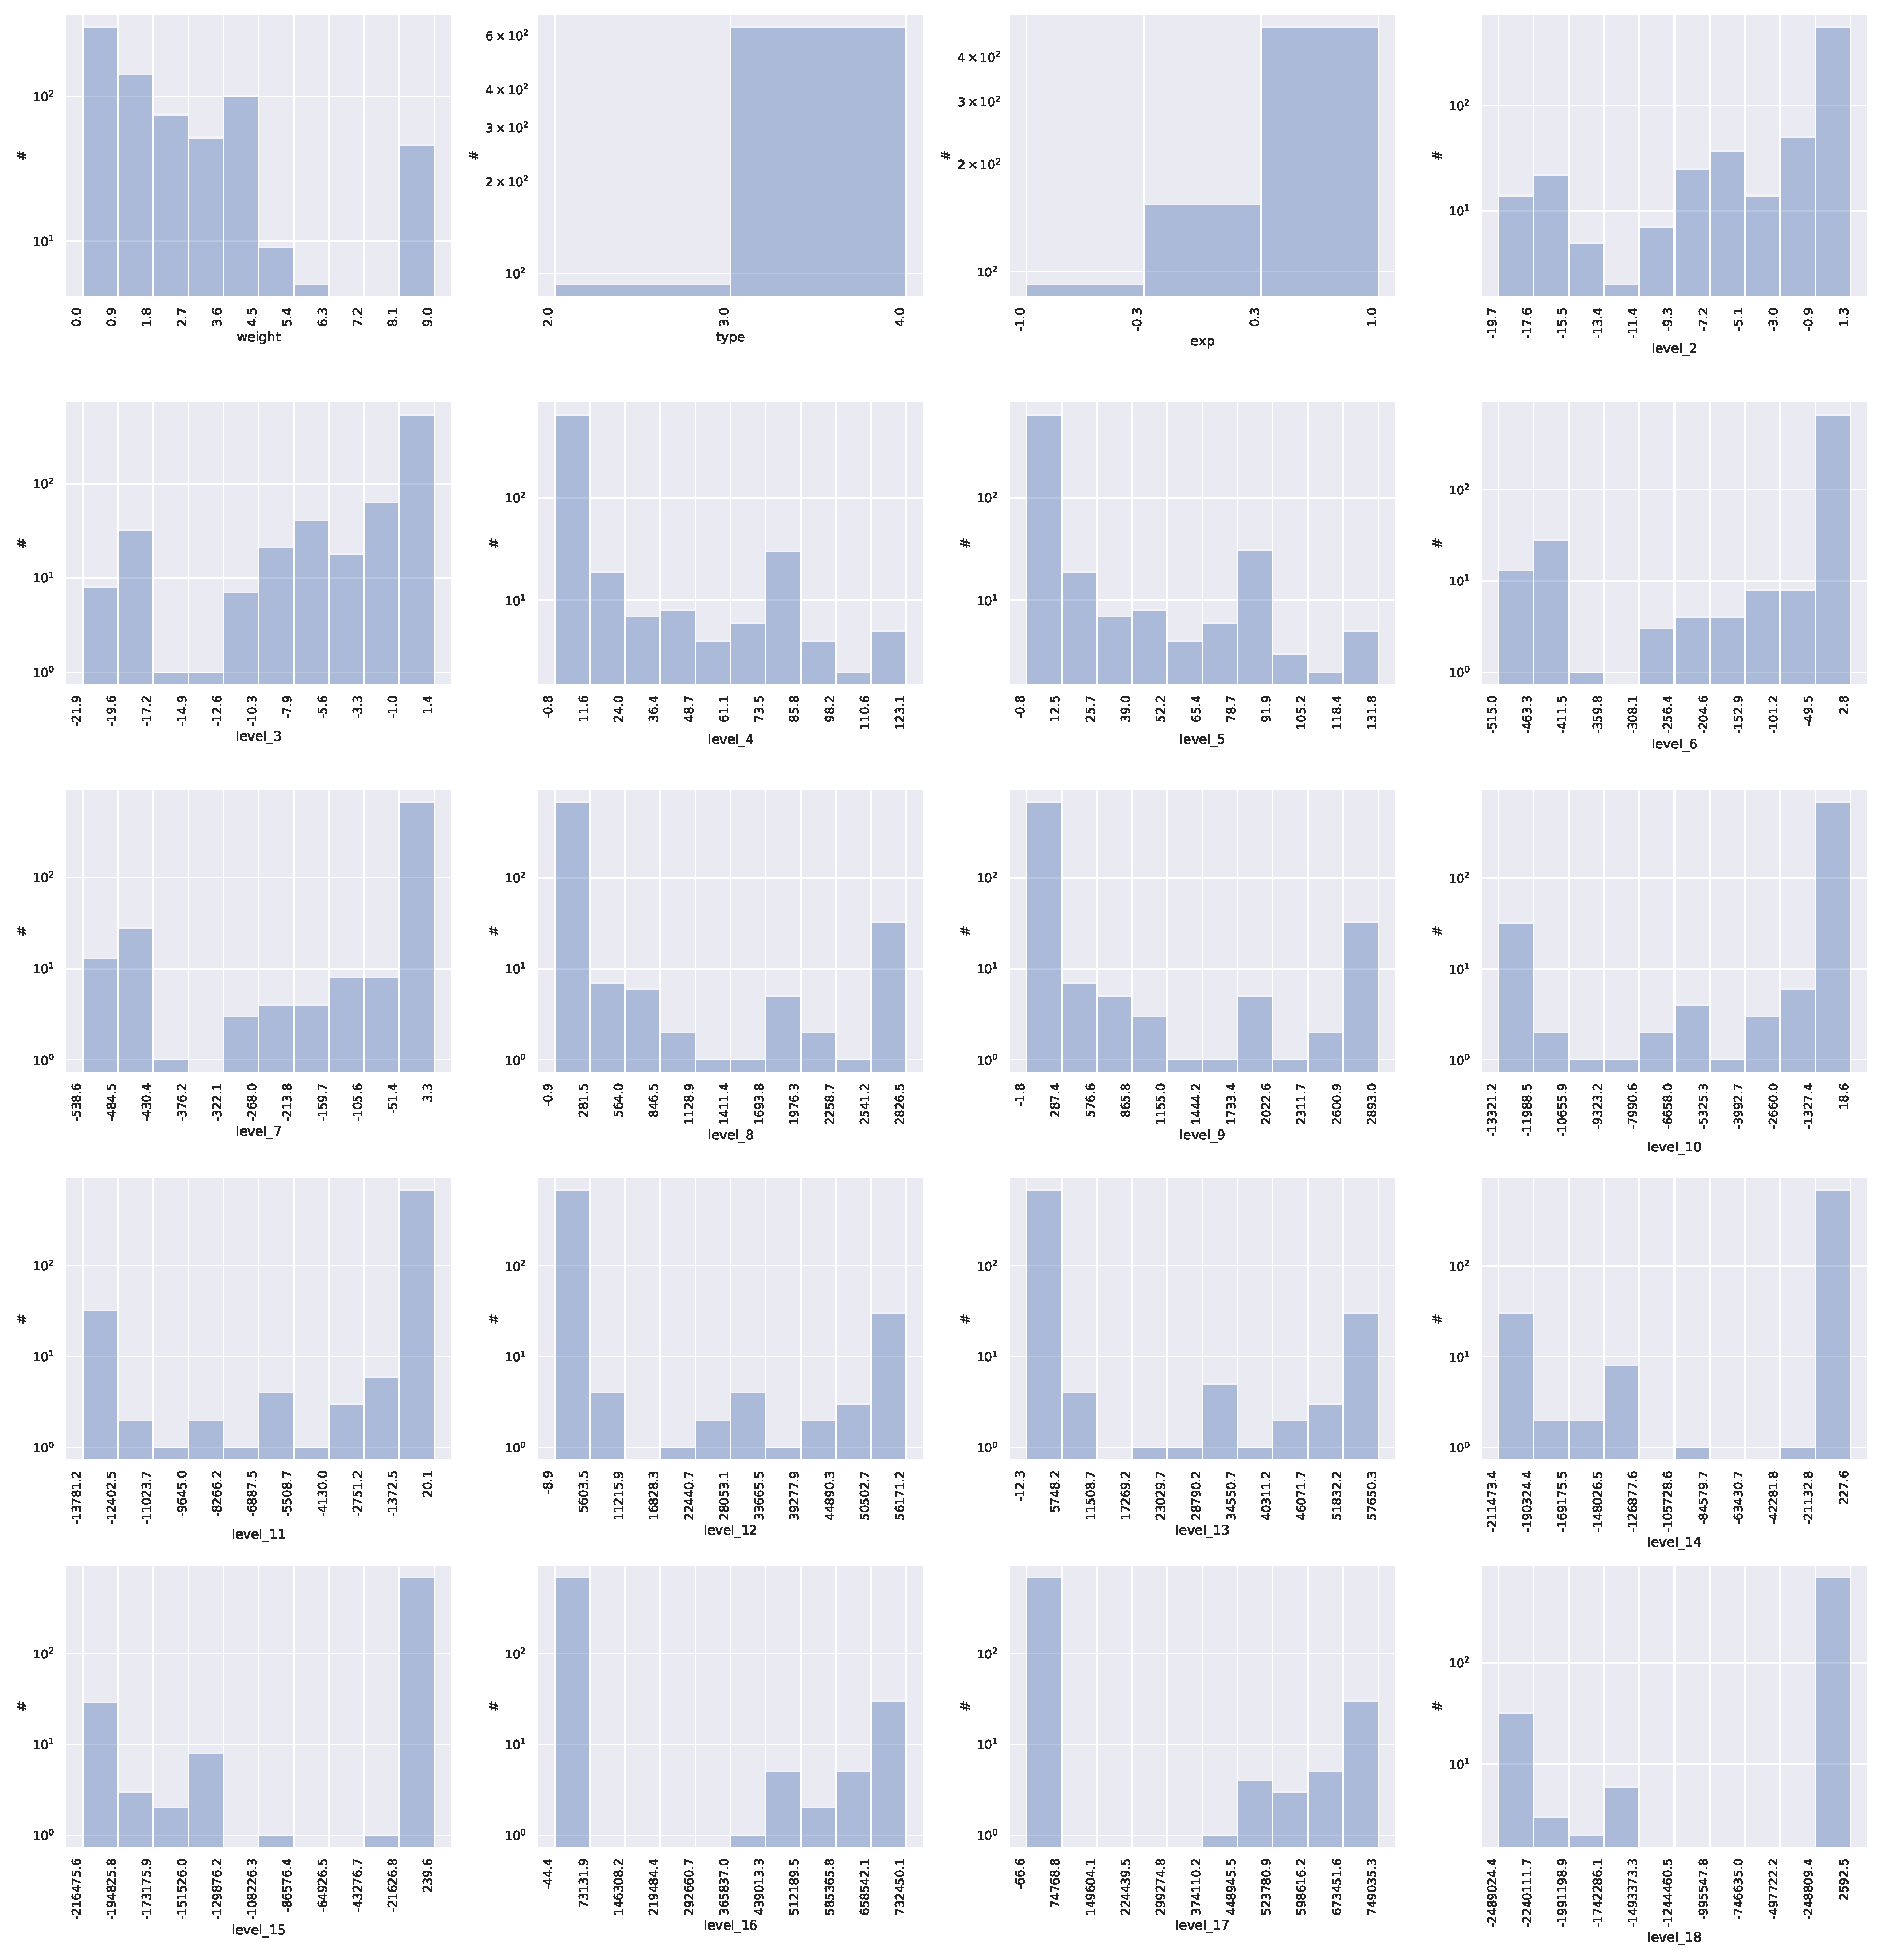
\includegraphics[width=0.4\textwidth]{img/dataset-distribution_full}
  \caption{Distribution of the variables in the dataset.}
  \label{fig:eda:distr_full}
\end{figure}
The distribution of the samples is summarised in \Cref{fig:eda:distr_full}: we
digitised each variable in at most 10 bins representing left-closed intervals
(i.e. $[a, b)$) between the values reported on the x-axis.
As we can see the distributions present a lot of outlying samples which may
lead to a ``artificially too small'' variance on the determination of the
coefficients of the regression.
The outliers are however mainly present in the distribution of the variables for which \texttt{weight} $\ge 1.5$.
\begin{figure}[htbp]
  \centering
  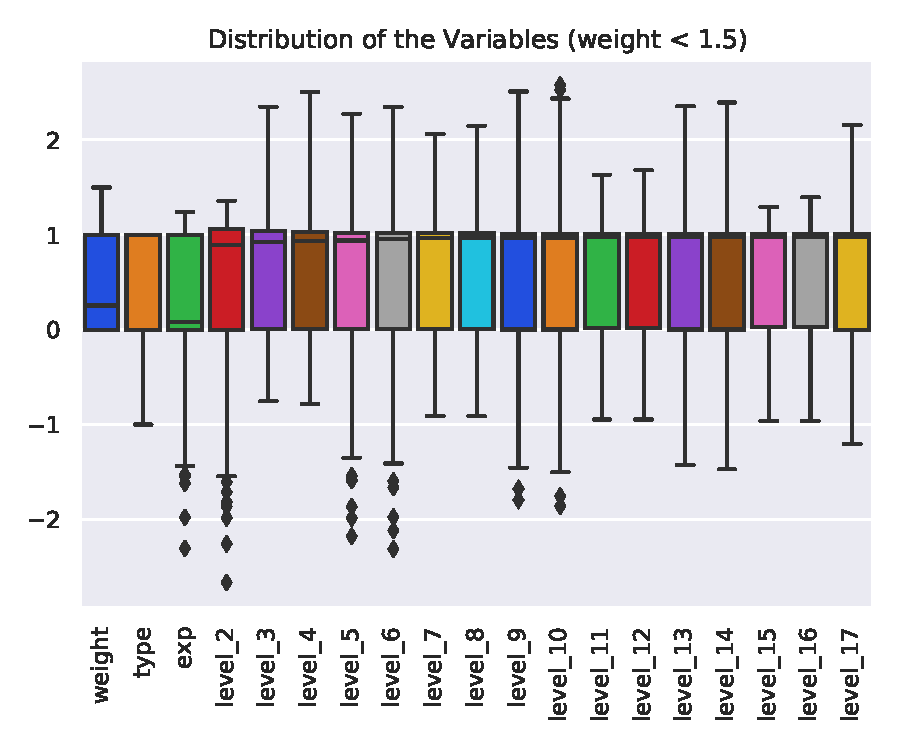
\includegraphics[width=0.4\textwidth]{img/dataset-distribution_box_low}
  \caption{Distribution of the variables for \texttt{weight} $< 1.5$.}
  \label{fig:eda:low_weight}
\end{figure}
In fact if we consider \texttt{weight} $< 1.5$ the variables are more
reasonably distributed, and might be easier to train in a following regression
analysis, as we show in \Cref{fig:eda:low_weight}.

\subsection{Correlations}\label{sec:eda:corr}

Following the outliers detection analysis, we first notice that for different
ranges of the \texttt{weight} variable, only certain types of oscillations are
present.
\begin{table}[htbp]
\centering
\begin{tabular}{@{}cccc@{}}
\toprule
                 &               & \multicolumn{2}{c}{\textbf{weight}} \\
\textit{range}   & \textit{type} & \textit{mean}  & \textit{variance}  \\
\midrule
weight $\ge 1.5$ & 4             & 4.03           & 5.13               \\
\midrule
\multirow{2}{*}
{weight $< 1.5$} & 2             & 0              & 0                  \\
                 & 4             & 0.58           & 0.21               \\
\bottomrule
\end{tabular}%
\caption{Type of oscillations per weight range.}
\label{tab:eda:weight}
\end{table}
In fact, in \Cref{tab:eda:weight} we show that for higher weights there is only
one type of oscillations in the dataset, while for lower weights the type 2
oscillation implies \texttt{weight} $= 0$ identically.

This in turns may also be reflected in the correlation between the variables.
This is defined for each possible couple of variables as the ration between
their covariance and the product of their separate standard deviations.
In \Cref{fig:eda:corr} we show the different correlation factors in a graphical
representation.
\begin{figure}[htbp]
  \centering
  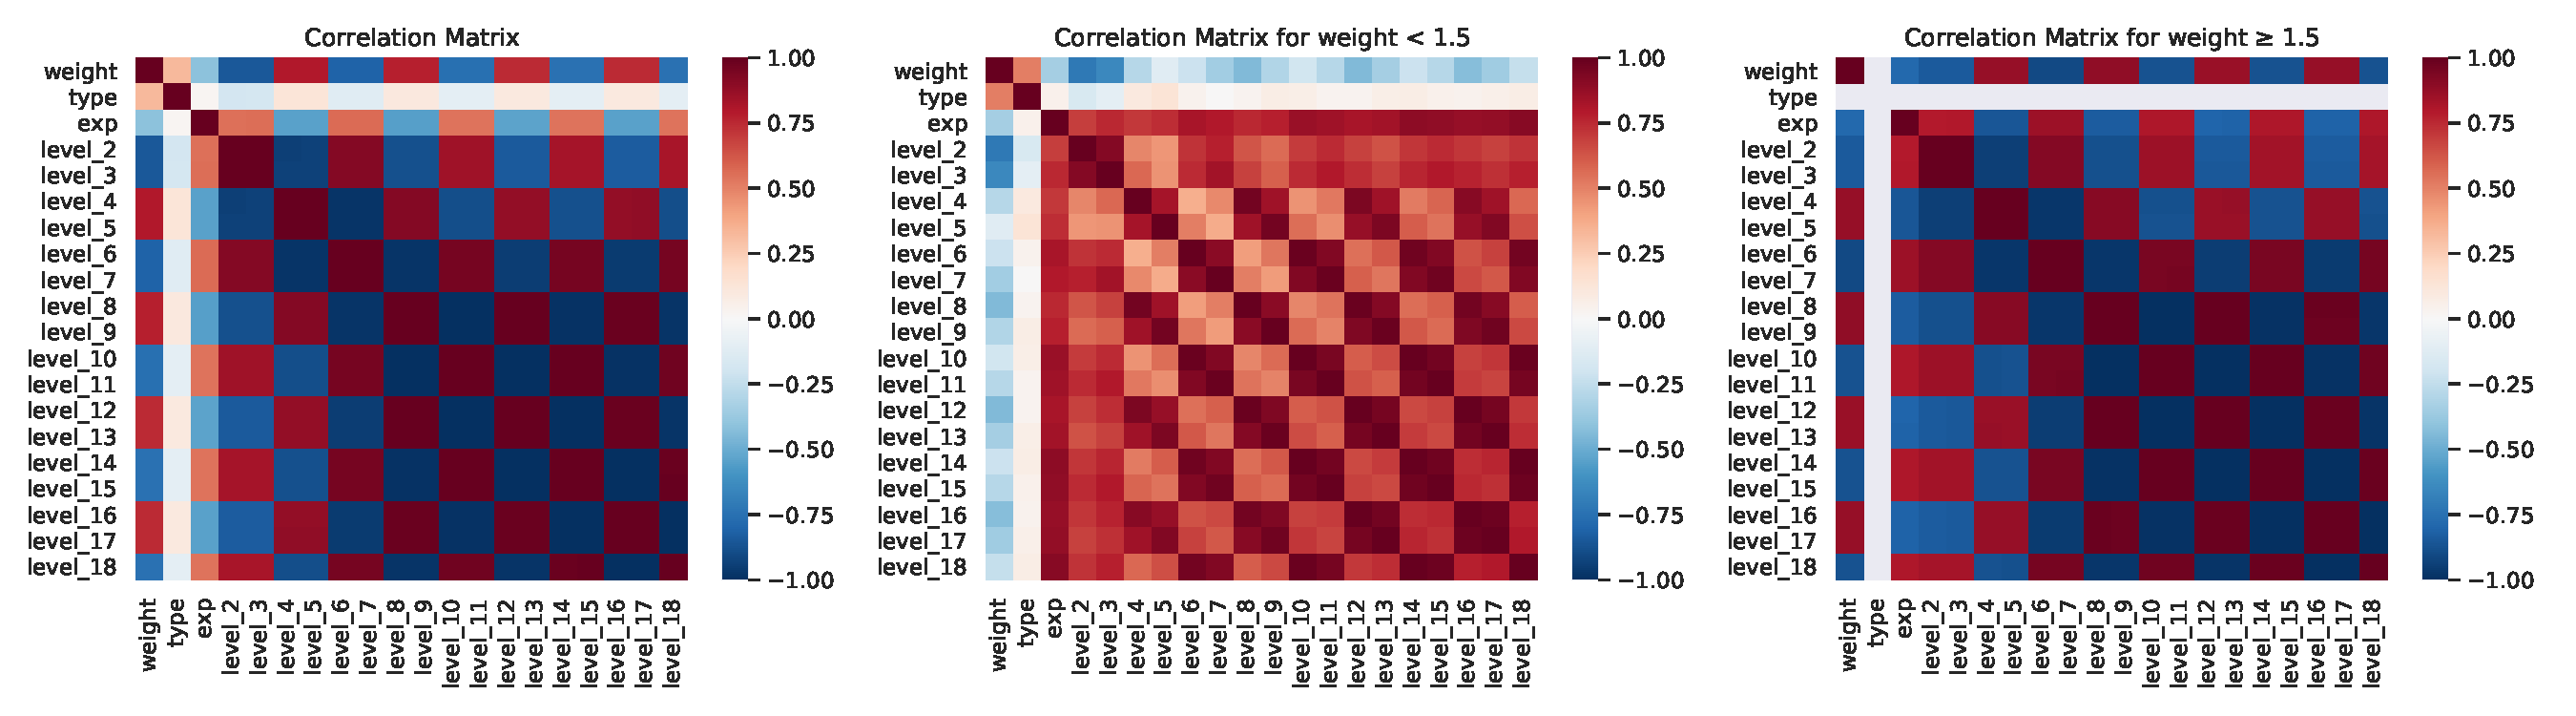
\includegraphics[width=0.4\textwidth]{img/corr-mat}
  \caption{Correlation matrix of the variables.}
  \label{fig:eda:corr}
\end{figure}
As expected, the truncation levels are strongly correlated among themselves and
with the \texttt{weight} variable.
Though milder, there is also a good correlation of the variables with the
labels we intend to predict (\texttt{exp}), while the \texttt{type} variable
seems to be completely uncorrelated (this may however be due to the fact of
being categorical: a linear regression might be more suitable to do statistical
inference on it).

\subsection{Principal Components Analysis}\label{sec:eda:pca}

We perform the Principal Components Analysis (PCA) of the truncation levels to
study their properties and their distribution.
We first study all its components using the Singular Value Decomposition (SVD)
of the matrix holding samples over the rows and the truncation levels over the
columns (it is a rectangular matrix and as such cannot be strictly diagonalised
to perform spectral analysis).
In \Cref{fig:eda:pca} we show the variance explained by each principal
component of the matrix (i.e.\ the fraction of variance of the total set
retained by considering only the selected component).
\begin{figure}[htbp]
  \centering
  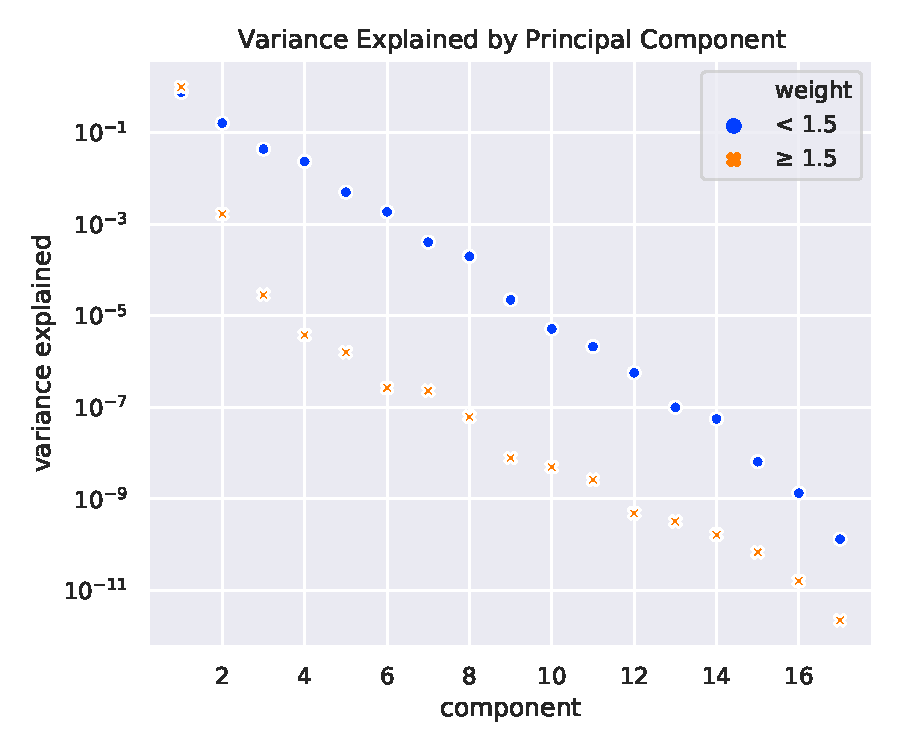
\includegraphics[width=0.4\textwidth]{img/pca-variance-explained}
  \caption{Variance explained by the principal components of the truncation levels (log scale).}
  \label{fig:eda:pca}
\end{figure}

The analysis was performed splitting the dataset over ranges of the
\texttt{weight} variable and shows that for lower weights the first two
principal components account for more than 90\% of the total variance of the
values, while for larger weights almost 100\% of the variance is explained by
the first component.
This reflects the distribution of the variables in the dataset: larger weights
contain a very large amount of outliers and have larger variance with respect
to lower weights, thus it might be enough to project the values of the
truncation levels over the line which contains most of the deviation to
reproduce a meaningful distribution.

\subsection{K-Means Clustering}\label{sec:eda:kmeans}

Finally we perform an unsupervised clustering analysis.
The main idea is to infer a structure in the data which may be able to
``automatically'' reproduce the labels (i.e.\ the \texttt{exp} column) without
regression.
In other words we study the distribution of the truncation levels and fit it in
3 clusters representing the 3 integer values of the labels.
In the ideal scenario there should be a 1:1 relation between the labels of the
cluster centroids and the labels in the \texttt{exp} variable. Unfortunately
the cluster analysis of the truncation levels over the entire dataset
highlighted no particular structure in the data and turned out inconclusive.

We then performed the same analysis splitting the dataset in different ranges
of the \texttt{weight} variable, standardising the data for \texttt{weight} $<
1.5$ and robustly scaling (i.e.\ scaling according the interquartile range)
samples for which \texttt{weight} $\ge 1.5$.
Based on the results of \Cref{sec:eda:pca}, in \Cref{fig:eda:kmeans} we used
the principal components of the truncation levels to plot the distribution of the clusters and the \texttt{exp} labels.
\begin{figure}[htbp]
  \centering
  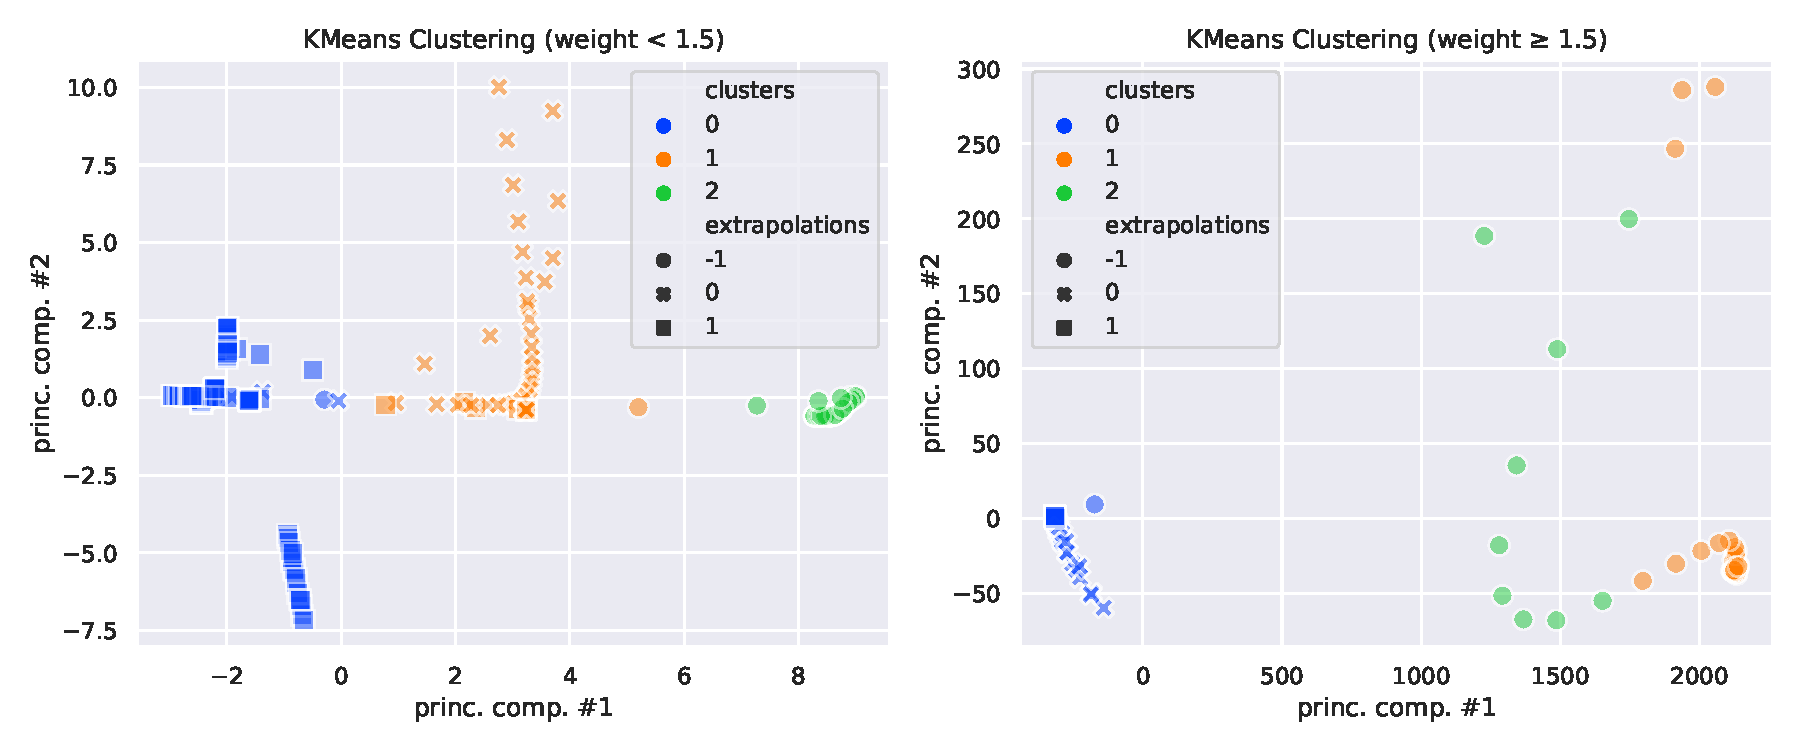
\includegraphics[width=0.475\textwidth]{img/kmeans-clusters}
  \caption{K-Means clusters and \texttt{exp} labels plotted using the principal
  components for visualisation purposes.}
  \label{fig:eda:kmeans}
\end{figure}
As we can see, recognising a structure is challenging when \texttt{weight} $\ge
1.5$ and in fact different \texttt{exp} (or ``extrapolation'') labels generally
belong to different clusters.
However the case \texttt{weight} $< 1.5$ seems to be more accurate and shows
that in general we can recognise a structure in the data.
\begin{table}[htbp]
\centering
\begin{tabular}{@{}cccc@{}}
\toprule
                     &              & \multicolumn{2}{c}{\textbf{weight}}   \\
\midrule
\textit{clusters}    & \textit{exp} & \textit{$< 1.5$} & \textit{$\ge 1.5$} \\
\midrule
\multirow{3}{*}
{average label} & -1 & 1.84             & 1.13               \\
                     & 0            & 0.92             & 0.00               \\
                     & 1            & 0.02             & 0.00               \\
\bottomrule
\end{tabular}%
\caption{Average cluster label per weight range.}
\label{tab:eda:kmeans}
\end{table}
In \Cref{tab:eda:kmeans} we recognise that there is a distinguishable relation
between the extrapolation column and the average cluster label in the group
when \texttt{weight} $< 1.5$, while in general there is a superposition of
labels when \texttt{weight} $\ge 1.5$ (it seems that there are only 2
recognisable clusters).
